\chapter{近似算法}
\raggedright%网络流之图像分割的老哥用了个\centering害人不浅
\begin{introduction}
	\item 近似算法介绍
	\item 顶点覆盖
	\item 任务调度
	\item 最小带权覆盖
	\item MAX-K-SAT
\end{introduction}

本章讲述了NPC问题的一些近似算法及其质量分析。

\section{近似算法介绍}

\subsection{引入与定义}

求解NPC问题的思路通常包括:
\begin{enumerate}
	\item 设计通用的指数级时间复杂度算法
	\item 针对特例设计多项式时间复杂度算法
	\item 根据问题特点设计启发式算法,或借用元启发式算法的框架求解(如蚁群、遗传、退火等算法)
	\item 设计近似算法
\end{enumerate}
其中设计近似算法时便要求时间复杂度是多项式级,得到的解可以保证与最优解比差别有限,具体定义如下。

\begin{definition}{近似算法}{approximation-algorithm:15Ln-ApproximationAlgorithm}
	对一个最小最优问题(最大最优则变为大于号)有多项式级时间复杂度,并对任意实例均有$ALG\leqslant \alpha \cdot OPT$,其中$\alpha$为一个常数,则称该算法为此问题的近似算法。(ALG为该算法结果的质量,OPT为最优解的质量)
\end{definition}

\subsection{近似算法常用证明方法}

\begin{figure}[htb]
	\centering
	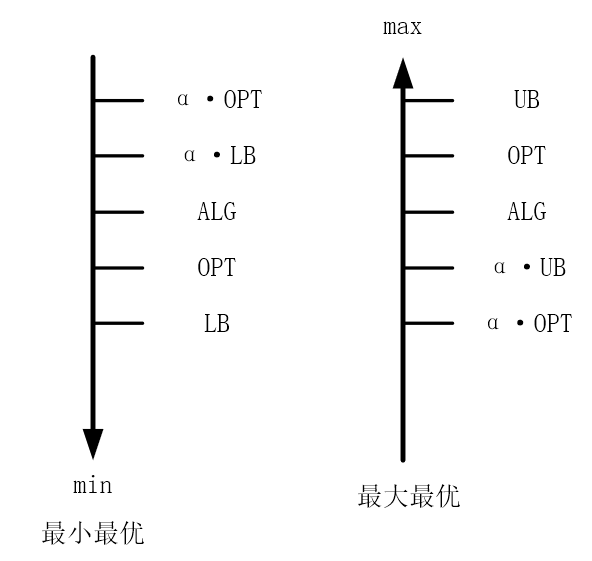
\includegraphics[scale=0.3]{image/Ln15-ApproximationAlgorithm1.png}
	\caption{近似算法证明思路} \label{proof:Ln15-ApproximationAlgorithm}
\end{figure}

\subsubsection{最小最优证明}
一般利用\autoref{proof:Ln15-ApproximationAlgorithm}的证明思路,首先找到OPT下界LB,证明$OPT\geqslant LB$,再想办法证明$ALG\leqslant \alpha \cdot LB$,从而得到$ALG\leqslant \alpha \cdot OPT$,即可证明该近似算法的正确性。
\subsubsection{最大最优证明}
同样利用\autoref{proof:Ln15-ApproximationAlgorithm}的证明思路,首先找到OPT上界UB,证明$OPT\leqslant UB$,再想办法证明$ALG\geqslant \alpha \cdot UB$,从而得到$ALG\geqslant \alpha \cdot OPT$,即可证明该近似算法的正确性。



\section{顶点覆盖}

本节将介绍一个顶点覆盖的近似算法。

\subsection{问题描述}

\begin{definition}{顶点覆盖问题}{vertex-cover:15Ln-ApproximationAlgorithm}
	对于给定的图$(V,E)$,找到一个点集$S\subset V$,使得该图所有边都至少有一个端点在点集S中。
\end{definition}

\subsection{算法描述}

算法步骤如下:
\begin{enumerate}
	\item 找到极大匹配M,相关定义如下:
	\begin{definition}{匹配}{matching:15Ln-ApproximationAlgorithm}
		给定一个图G,在G的一个子图M中,任意两边都没有相同的端点,且每个点都有边相连。
	\end{definition}
	\begin{definition}{极大匹配}{maximal-matching:15Ln-ApproximationAlgorithm}
		一个匹配无法再增加任何点和边,则称之为极大匹配。
	\end{definition}
	\item 输出M中的所有点作为解的点集S
\end{enumerate}

\subsection{正确性证明}

\begin{proposition}{求证}{proof1:15Ln}
该算法始终有$ALG\leqslant 2\cdot OPT$,在该问题中OTP即为最优解点的数量,ALG即为算法求解的点的数量。
\end{proposition}
证明:
\begin{enumerate}
	\item 证明$OPT\geqslant |M|$(其中|M|为极大匹配的边数):对于M中任意一条边,其必定至少有一点在OPT中,否则这条边就未被覆盖,与顶点覆盖的要求矛盾。故$OPT\geqslant |M|$
	\item 证明$ALG=2\cdot |M|$:极大匹配中任意一点度为1,故点的数量即为边的数量的两倍,得证$ALG=2\cdot |M|$。
	\item 根据上述证明可以得到$2\cdot OPT\geqslant 2\cdot|M|=ALG$,得证$ALG\leqslant 2\cdot OPT$
\end{enumerate}
	
\section{任务调度}

\subsection{问题描述}
定义任务$T$为集合$\{t_1,t_2,\ldots,t_n\}$,有$m$台机器$\{M_1,M_2,\ldots,M_m\}$,而一任务调度即将任务$T$中的所有任务分配给这$m$台机器,假设对第$i$台机器,设其被分配的任务为集合$A(i),i\in [1,m]$,则其执行任务的总时间可定义为
\begin{equation*}
	T_i=\sum_{j\in A(i)} t_j
\end{equation*}
所有机器并行执行任务,则完成所有任务的时间$T$可表示为
\begin{equation*}
	T=\max_{i=1}^{m} T_i
\end{equation*}
要求寻找一个算法,使得$T$尽可能的小,设实际最优解为$T_0$

该问题为$NP-hard$问题,所以无法在多项式找出最优解,以下给出的均为近似算法,并讨论解与最优解的关系。

\begin{example}
	假设有6个任务,其所需执行时间依次为2,3,4,6,2,2,有三台机器,则其最优解$T_0=7$。
\end{example}

\subsection{贪心算法一[在线算法]}
该问题最直接的思路就是贪心算法,将依次取$t_1,t_2,\ldots,t_n$,让$m$台机器执行,每次挑选的机器的$T_i$都是最小的,即每次$t_i$都加入到当前负载$T_k$最小的机器,设该算法给出的近似解为$T_1^*$

算法的伪代码如下

\begin{algorithm}
	\DontPrintSemicolon{}
	\KwResult{the minimum $T_1^*$}
	\Begin{
		Start with no tasks assigned\\
		Set $T_i=0$ and $A(i)=\{\}$ for all machines $M_i$
		\ForEach{$j \in [1,n]$}{
			Let $M_i$ be a machine which $T_i$ the minimum at present\\
			Aissign task j to machine $M_i$\\
			Set $A(j)=A(i)\cup \{j\}$\\
			Set $T_j=T_i+t_j$
		}
	}
	\caption{Greedy-Algorithm1}\label{greedy1-algo}
\end{algorithm}

该算法在所给出的例子中运行的结果如下图所示,这里给出的近似解为$T_1^*=6+2=8$
\begin{figure}[hbt]
	\centering
	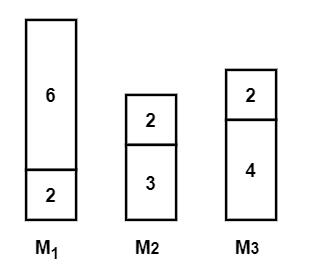
\includegraphics{image/greedy1-result.jpg}
	\caption{贪心算法一的结果}\label{fig:greedy1-result}
\end{figure}

实际上我们可以证明,$T_1^*$和$T_0$有如下关系:
\begin{equation*}
	T_1^*\leq 2T_0
\end{equation*}

证明首先需要用到两个显而易见的定理。
\begin{theorem}{}{label-for-the1}
	最优解$T_0$不可能比所有任务在所有机器执行的平均时间还小,即
	\begin{equation*}
		T_0\geq \frac{\sum_j t_j}{m}
	\end{equation*}
\end{theorem}

\begin{theorem}{}{label-for-the2}
	最优解$T_0$不可能比任务时间最长的那个任务的时间小,即
	\begin{equation*}
		T_0\geq \max_j t_j
	\end{equation*}
	因此$T_0$会大于等于任一$t_i$。
\end{theorem}

进一步假设由该贪婪算法所得到的$T_1^*$由第i台机器产生,如下图所示
\begin{figure}[hbt]
	\centering
	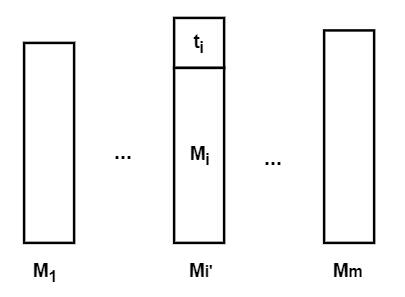
\includegraphics{image/greedy1-proof.jpg}
	\caption{贪心算法一近似比的证明}\label{fig:greedy1-proof}
\end{figure}

\begin{proof}
	由定理2可知,最上面的那个任务$t_i$的执行时间不会比$T_0$更大,即
	\begin{equation*}
		t_i \leq \max_j t_j \leq T_0
	\end{equation*}
	而$M_i$是所执行的剩下任务的总时间,根据贪婪算法的执行的策略,会导致在使$M_i$执行最上面的那个任务之前,剩下的任务的时间之和是最小的,由定理1可知,该部分时间和不会超过$T_0$,即
	\begin{equation*}
		M_i \leq AVG \leq T_0
	\end{equation*}
	因此,$T_1^*\leq 2T_0$成立。
\end{proof}

\subsection{贪心算法二[先排序再贪心]}
针对贪心算法一,一个很自然的改进措施,将所有任务按照从大到小的时间进行排序,然后再执行贪心算法一。

算法的伪代码如下

\begin{algorithm}
	\DontPrintSemicolon{}
	\KwResult{the minimum $T_2^*$}
	\Begin{
		Start with no tasks assigned\\
		Sort tasks in decreasing order of processing time $t_j$ \\
		Assume that $t_1 \geq t_2 \geq \ldots \geq t_n$
		Set $T_i=0$ and $A(i)=\{\}$ for all machines $M_i$
		\ForEach{$j \in [1,n]$}{
			Let $M_i$ be a machine which $T_i$ the minimum at present\\
			Aissign task j to machine $M_i$\\
			Set $A(j)=A(i)\cup \{j\}$\\
			Set $T_j=T_i+t_j$
		}
	}
	\caption{Greedy-Algorithm2}\label{greedy2-algo}
\end{algorithm}

该算法在所给出的例子中运行的结果如下图所示,这里给出的近似解为$T_2^*=3+2+2=7$
\begin{figure}[hbt]
	\centering
	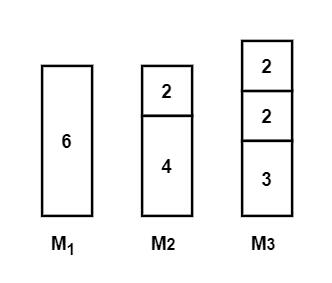
\includegraphics{image/greedy2-result.jpg}
	\caption{贪心算法二的结果}\label{fig:greedy2-result}
\end{figure}

实际上我们可以证明,$T_2^*$和$T_0$有如下关系:
\begin{equation*}
	T_1^*\leq \frac{3}{2} T_0
\end{equation*}

进一步假设由该贪婪算法所得到的$T_2^*$由第i台机器产生,如下图所示
\begin{figure}[hbt]
	\centering
	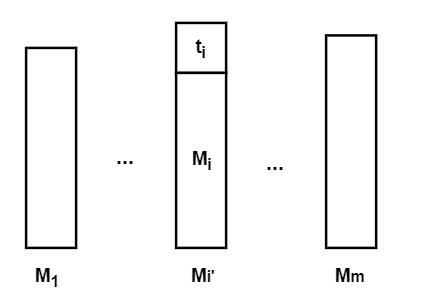
\includegraphics{image/greedy2-proof.jpg}
	\caption{贪心算法二近似比的证明}\label{fig:greedy2-proof}
\end{figure}

\begin{proof}
	首先,如果任务数$n$小于等于机器数$m$,那么显然有$T_2^*=T_0$,结论成立。

	如果任务数$n$大于机器数$m$,则有$T_0 \geq 2t_{m+1}$,因为一开始第$1$到第$m$个任务会被依次放在第$1$到第$m$台机器上,而第$m+1$个任务必然会放在这几个任务之后执行,而由于任务已经按降序排序,故第$m+1$个任务放好之后,必然会大于$2t_{m+1}$,而它必然小于等于$T_0$,即$T_0 \geq 2t_{m+1}$,则有
	\begin{equation*}
		t_{m+1} \leq \frac{1}{2}T_0
	\end{equation*}
	
	在图中,最上面的那个任务$t_i$的执行时间不会比$t_{m+1}$更大(因为序号在m+1后面),即
	\begin{equation*}
		t_i \leq t_{m+1} \leq \frac{1}{2}T_0
	\end{equation*}
	而$M_i$是所执行的剩下任务的总时间,根据贪婪算法的执行的策略,会导致在使$M_i$执行最上面的那个任务之前,剩下的任务的时间之和是最小的,由定理1可知,该部分时间和不会超过$T_0$,即
	\begin{equation*}
		M_i \leq AVG \leq T_0
	\end{equation*}
	因此,$T_2^*\leq \frac{3}{2}T_0$成立。

	综上所述,$T_2^*\leq \frac{3}{2}T_0$成立。
\end{proof}

\subsection{补充}
实际上,对于算法二而言,$\frac{3}{2}$并非下确界,实际上的下确界为
\begin{equation*}
	T_2^*\leq \frac{4}{3} T_0
\end{equation*}

此处下确界的含义是,不可能再找到一个比它更小的正数满足上式。

进一步假设由该贪婪算法所得到的$T_2^*$由第i台机器产生,如下图所示
\begin{figure}[hbt]
	\centering
	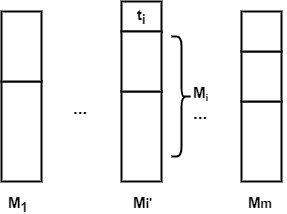
\includegraphics{image/greedy2-proof-4-3.jpg}
	\caption{贪心算法二近似比的证明}\label{fig:greedy2-proof-4-3}
\end{figure}

\begin{proof}
	首先,如果任务数$n$小于等于机器数$m$,那么显然有$T_2^*=T_0$,结论成立。

	然后,如果任务数$n$与机器数$m$的关系满足$n>2m$时,则有$T_0 \geq 3t_{2m+1}$,对于前$2m+1$个任务,由鸽笼原理,必有一个机器分到3个任务,而由于任务已经按降序排序,故第$2m+1$个任务放好之后,这个机器上的3个任务和必然会大于$3t_{2m+1}$,而它必然小于等于$T_0$,即$T_0 \geq 3t_{2m+1}$,则有
	\begin{equation*}
		t_{2m+1} \leq \frac{1}{3}T_0
	\end{equation*}
	
	在图中,最上面的那个任务$t_i$的执行时间不会比$t_{2m+1}$更大(因为序号在2m+1后面),即
	\begin{equation*}
		t_i \leq t_{2m+1} \leq \frac{1}{3}T_0
	\end{equation*}
	而$M_i$是所执行的剩下任务的总时间,根据贪婪算法的执行的策略,会导致在使$M_i$执行最上面的那个任务之前,剩下的任务的时间之和是最小的,由定理1可知,该部分时间和不会超过$T_0$,即
	\begin{equation*}
		M_i \leq AVG \leq T_0
	\end{equation*}
	因此,$T_2^*\leq \frac{4}{3}T_0$成立。

	最后,当$m<n \leq 2m$时,也不能得到$T_0$,只能得到$\frac{4}{3}T_0$,此部分证明复杂。

	综上所述,$T_2^*\leq \frac{4}{3}T_0$成立。
\end{proof}

\begin{example}
	假设有$2m+1$个任务,执行时间分别为$m$到$2m$和$m+1$到$2m$,求解贪心算法二的近似比。
\end{example}
该问题的特殊性使得其最优解可以凭直觉得到为$3m+2$,调度策略如下图所示。
\begin{figure}[hbt]
	\centering
	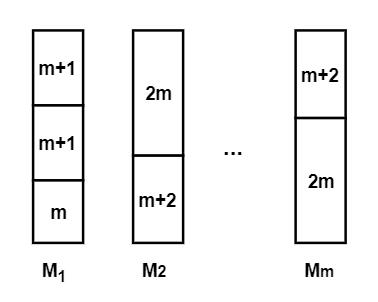
\includegraphics{image/example-problem-opt-solve.jpg}
	\caption{最优解调度}\label{fig:example-problem-opt-solve}
\end{figure}

而利用贪婪算法二得出的近似解$T_2^*$则为$4m+1$,证明如下。
\begin{proof}
	贪心算法二调度策略如下表所示。
	% Please add the following required packages to your document preamble:
	% \usepackage{multirow}
	\begin{table}[]
	\begin{tabular}{cccccccc}
	\hline
	$M_1$                  & $M_2$                  & $M_3$                   & $M_4$                   & ...                                       & $M_{m-1}$            & $M_m$                & m的奇偶性 \\ \hline
	\multirow{2}{*}{$2m$}  & \multirow{2}{*}{$2m$}  & \multirow{2}{*}{$2m-1$} & \multirow{2}{*}{$2m-1$} & \multicolumn{1}{c|}{\multirow{2}{*}{...}} & $2m-\frac{m}{2}+1$   & $2m-\frac{m}{2}+1$   & 偶数m   \\ \cline{6-8} 
						   &                        &                         &                         & \multicolumn{1}{c|}{}                     & $2m-\frac{m+1}{2}+2$ & $2m-\frac{m+1}{2}+1$ & 奇数m   \\ \hline
	\multirow{2}{*}{$m+1$} & \multirow{2}{*}{$m+1$} & \multirow{2}{*}{$m+2$}  & \multirow{2}{*}{$m+2$}  & \multicolumn{1}{c|}{\multirow{2}{*}{...}} & $2m-\frac{m}{2}$     & $2m-\frac{m}{2}$     & 偶数m   \\ \cline{6-8} 
						   &                        &                         &                         & \multicolumn{1}{c|}{}                     & $2m-\frac{m+1}{2}$   & $2m-\frac{m+1}{2}+1$ & 奇数m   \\ \hline
	$m$                    &                        &                         &                         &                                           &                      &                      &       \\ \hline
	4m+1                   & 3m+1                   & 3m+1                    & 3m+1                    & ...                                       & 3m+1                 & 3m+1                 &      
	\end{tabular}
	\end{table}
	
	贪心算法二的调度顺序为从第一排从左到右,第二排从右到左,第三排剩一个m,由表可以得到最大时间为$4m+1$。
\end{proof}

因此贪心算法的近似比为$\lim_{m\to \infty}\frac{4m+1}{3m+2}=\frac{4}{3}$

更一般的,对于算法解$ALG$和最优解$OPT$,有$\frac{ALG}{OPT} \leq \frac{4}{3}-\frac{1}{3m}$。



\section{最小带权覆盖}

本节将介绍一个最小带权覆盖的近似算法。

\subsection{问题描述}

\begin{definition}{最小带权覆盖问题}{weighted-vertex-cover:15Ln-ApproximationAlgorithm}
	对于给定的图$(V,E)$,各个点有权重w,找到一个点集$S\subset V$,使得该图所有边都至少有一个端点在点集S中,且S中所有点的权重之和比所有可行的解都小。
\end{definition}

\subsection{算法描述}

算法步骤如下:
\begin{enumerate}
	\item 将原问题建模为线性规划问题:
	原问题是$\forall e=(u,v)\epsilon E$,有$v\epsilon S$或$u\epsilon S$,求$\min \sum\limits_{v\epsilon G} x_vw_v$其中
	\[
		x_v = \begin{cases}
			0 & v\notin S \\
			1 & v\epsilon S
		\end{cases}
	\]\\
	将其转化为线性规划问题,可变为:
	\[
		\begin{cases}
			x_v^*+x_u^*\geqslant 1 			   &\forall e=(u,v)\epsilon E\\
			x_v^*\geqslant 0	   			   &\forall v\epsilon G, x_v\epsilon [0,1]\\
			\min \sum\limits_{v\epsilon G} x_v^*w_v
		\end{cases}
	\]
	\item 使用线性规划求解器求解,再将得到的解转化为原问题的解:
	\[
		x_v=\begin{cases}
			0 &x_v^*<0.5\\
			1 &x_v^*\geqslant 0.5
		\end{cases}
	\]
\end{enumerate}

\subsection{正确性证明}

\begin{proposition}{求证}{proof2:15Ln}
	该算法得到的解是一个顶点覆盖
\end{proposition}
证明:
	因为$\forall e=(u,v)\epsilon E,x_v^*+x_u^*\geqslant 1$,故$x_v^*\geqslant 0.5$或$x_u^*\geqslant 0.5$,故$x_v$和$x_u$至少有一个为1,即至少有一点覆盖该边e。得证该算法得到的解是一个顶点覆盖。
\begin{proposition}{求证}{proof3:15Ln}
	$ALG\leqslant 2\cdot OPT$
\end{proposition}
证明:
	$OPT\geqslant \sum\limits_{v\epsilon G} x_v^*w_v^*$,而又有$x_v\leqslant 2\cdot x_v^*$,故有
	$ALG=\sum\limits_{v\epsilon G} x_vw_v\leqslant 2\cdot \sum\limits_{v\epsilon G} x_v^*w_v^*\leqslant 2\cdot OPT$,得证。

\section{MAX-K-SAT}

本节将介绍三个MAX-K-SAT的算法。

\subsection{问题描述}

\begin{definition}{K-STA问题}{K-SAT:15Ln-ApproximationAlgorithm}
	对于一个公式F,其由n个子句${C_1,\cdots ,C_n}$与运算构成,每个子句又恰好由三个文字或运算构成,即$C_i=L_{i1}\bigvee L_{i2}\bigvee L_{i3}$。每个文字的值取一个变元$X_i$的值或取其非。求一组变元赋值方案,使得公式F为真。
\end{definition}

\begin{definition}{MAX-K-SAT问题}{max-K-SAT:15Ln-ApproximationAlgorithm}
	对于一个K-SAT问题,求一组赋值方案使得值为真的子句数量最多。
\end{definition}

\subsection{随机算法}

\subsubsection{算法描述}

对所有文字$X_i (i=1,\cdots,n)$等概率随机赋值
\[
	X_i=\begin{cases}
		0 &P=0.5\\
		1 &P=0.5
	\end{cases}
\]

\subsubsection{算法分析}
\begin{itemize}
	\item $P(C_i=1)=1-\frac{1}{2^K} $
	\item 故有$E(ALG)=E(\sum\limits_{i=1}^n C_i)=\sum\limits_{i=1}^n E(C_i)=n\cdot (1-\frac{1}{2^K})$
	\item 又由$ALG\leqslant OTP\leqslant n$
	\item 可得$\frac{E(ALG)}{OPT}\geqslant \frac{E(ALG)}{n}=1-\frac{1}{2^K}\geqslant 0.5$
	\item 注意这里的分子并不是ALG,而是ALG的期望
\end{itemize}

\subsection{确定性贪心算法}

\subsubsection{算法描述}

对于随机算法有该递推式:$E(ALG1)=\frac{1}{2}E(ALG1|X_i=0)+\frac{1}{2}E(ALG1|X_i=1)$。
本算法便基于这一点让本算法的E(ALG2)不小于随机算法的E(ALG1),记变元数为m。

\begin{algorithm}
\For{$i=1$\KwTo$m$}{
	\If{$E(ALG1|X_i=0,X_{i-1},\cdots,X_1)>E(ALG1|X_i=1,X_{i-1},\cdots,X_1)$}{$X_i=0$}
	\Else{$X_i=1$}
}
\end{algorithm}

\subsubsection{算法分析}
由算法描述可知,对任何$i=1,\cdots,m$都有
\begin{displaymath}
	E(ALG2|X_{i-1},\cdots,X_1)=max(E(ALG1|X_i=0,X_{i-1},\cdots,X_1),E(ALG1|X_i=1,X_{i-1},\cdots,X_1))	
\end{displaymath}
故有
\begin{displaymath}
E(ALG2)=max(E(ALG1|X_i=0),E(ALG1|X_i=1))\geqslant E(ALG1)
\end{displaymath}

\subsection{线性规划算法}

\subsubsection{算法描述}

在线性规划建模中,记$q_i$为$C_i$的值,$y_i$为$L_i$的值,$f_{ij}$为变元$x_i$在$C_i$中的符号。则变为线性规划问题
\[
	\begin{cases}
		q_i,y_i\epsilon [0,1]\\
		q_i\leqslant \sum\limits _{f_{ij}>0}y_j+\sum\limits _{f_{ij}<0}(1-y_j)\\
		\max \sum\limits_{i=1,\cdots,n}q_i
	\end{cases}
\]
线性规划求解完成后,取
\[
	x_i=\begin{cases}
		1 &P=y_i\\
		0 &P=1-y_i
	\end{cases}
\]

\subsubsection{算法分析}
线性规划求解完成后,对任一子句不妨假设其符号全为正,便于证明推导:
\begin{displaymath}
	\begin{split}
		&\because q_i\leqslant \sum\limits_{j=1,\cdots,K} y_j\\
		&\therefore 1-\frac{q_i}{K}\geqslant \frac{1}{K}\sum\limits_{j=1,\cdots,K}(1-y_j)\ \ \ \ (1)
	\end{split}
\end{displaymath}
故有
\begin{displaymath}
	\begin{split}
		P(C_i=1)&=1-\prod _{j=1}^K(1-y_j)\\
		&\geqslant[\frac{1}{K}\sum\limits_{j=1}^K(1-y_j)]^K\\
		(1)\Rightarrow &\geqslant 1-(1-\frac{q_i}{K})^K\\
		q_i\leqslant 1\Rightarrow &\geqslant q_i[1-(1-\frac{1}{K})^K]\\
		&\geqslant q_i(1-\frac{1}{e})
	\end{split}
\end{displaymath}
故有
\begin{displaymath}
	\begin{split}
		E(ALG)&=E(\sum\limits_{i=1}^n C_i)=\sum\limits_{i=1}^n E(C_i)\\
		&=(1-\frac{1}{e})\sum\limits_{i=1,\cdots,n}q_i\\
		&=(1-\frac{1}{e})\cdot OPT(LP)\\
		&\geqslant(1-\frac{1}{e})OPT
	\end{split}
\end{displaymath}
即$\frac{E(ALG)}{OPT}\geqslant 1-\frac{1}{e}$
